% \usepackage[singlelinecheck=false]{caption}
\usepackage{enumitem}
\usepackage{setspace}
% \onehalfspacing
% \usepackage[inner=1.0in, outer=1.0in, top=1.0in, bottom=1.0in]{geometry}
\hypersetup{
colorlinks = true,
linkcolor = blue,
filecolor = magenta,
urlcolor = cyan,
citecolor = blue
}

\usepackage{tikz}

% datasummary tables formatting
\usepackage{float}
\usepackage[normalem]{ulem}
\usepackage{tabularray}
\UseTblrLibrary{booktabs}
\UseTblrLibrary{siunitx}
\newcommand{\tinytableTabularrayUnderline}[1]{\underline{#1}}
\newcommand{\tinytableTabularrayStrikeout}[1]{\sout{#1}}
\NewTableCommand{\tinytableDefineColor}[3]{\definecolor{#1}{#2}{#3}}

% for rotating tables
\usepackage{pdflscape}
\usepackage{afterpage}

\usepackage{adjustbox}

\setcounter{secnumdepth}{3}

\documentclass[a4paper,12pt]{article}
\usepackage[utf8]{inputenc}
\usepackage[T1]{fontenc}
\usepackage{graphicx}
\usepackage{longtable}
\usepackage{wrapfig}
\usepackage{rotating}
\usepackage[normalem]{ulem}
\usepackage{amsmath}
\usepackage{amssymb}
\usepackage{capt-of}
\usepackage{hyperref}
\usepackage{amsmath,amsfonts,amsthm,amssymb}
\usepackage[singlelinecheck=false]{caption}
\captionsetup[subfigure]{singlelinecheck=on, labelfont=normalfont}
\captionsetup[figure]{labelfont=it}
\usepackage{graphicx}
\usepackage{rotating}
\usepackage{enumitem}
\usepackage{setspace}
\onehalfspacing
\usepackage[normalem]{ulem}
\usepackage{hyperref}
\hypersetup{
colorlinks = true,
linkcolor = blue,
filecolor = magenta,
urlcolor = cyan,
citecolor = blue
}

\usepackage{tikz}

% datasummary tables formatting
\usepackage{tabularray}
\usepackage{float}
\usepackage{graphicx}
\usepackage[normalem]{ulem}
\UseTblrLibrary{booktabs}
\UseTblrLibrary{siunitx}
\newcommand{\tinytableTabularrayUnderline}[1]{\underline{#1}}
\newcommand{\tinytableTabularrayStrikeout}[1]{\sout{#1}}
\NewTableCommand{\tinytableDefineColor}[3]{\definecolor{#1}{#2}{#3}}

% for rotating tables
\usepackage{pdflscape}
\usepackage{afterpage}
\usepackage{capt-of}% or use the larger `caption` package

\usepackage{natbib}
\bibliographystyle{apalike}
\setcounter{secnumdepth}{3}
\author{Dante Yasui}
\date{2025-06-19}
\title{Forced Removal or Moved to Opportunity?\\\medskip
\large Labor Market and Migration Effects of Japanese Internment}
\hypersetup{
 pdfauthor={Dante Yasui},
 pdftitle={Forced Removal or Moved to Opportunity?},
 pdfkeywords={migration, economic mobility, economic history},
 pdfsubject={Job market paper manuscript},
 pdfcreator={Emacs 29.1 (Org mode 9.6.6)}, 
 pdflang={English}}
\begin{document}

\maketitle

\begin{abstract}
  % Intro sentence
  During World War II a large scale forced migration of over 100,000
  Japanese American immigrants and their citizen children
  lead to relocation away from the West Coast.
  % Methods
  I analyse the effect that this forced relocation had
  on the post-war earnings of a linked sample of likely internees.
  My empirical strategy uses an individual-level panel of Japanese
  and Chinese men and women to compare earnings before and after internment.
  % Results
  I find that individuals who were likely interned experienced faster growth in
  earnings compared to their counterfactual earnings if they had not been
  interned.  
  % Mechanisms
  The possible mechaisms which might explain this seeming adaptation
  include occupational change and later migration decisions.
\end{abstract}

\section{Introduction}
In this paper, I explore the long-term migration patterns of Japanese Americans
who were forcibly relocated during World War II.
Specifically, I investigate whether geographic proximity to the internment camps
established by the War Relocation Authority (WRA)
influenced migration rates among the Japanese American population
in the decades following internment.
The central research question is
whether counties closer to these internment camps experienced a disproportionately higher rate of Japanese American migration compared to more distant counties.

The US government's internment policy displaced more than 100,000 Japanese Americans from their homes, 
primarily on the West Coast,
and placed them in camps scattered across remote areas of the Western US and Arkansas.
Following the war, 
efforts were made to disperse the Japanese American population more widely across the US,
often discouraging their return to prewar enclaves.
These policies highlight the need to examine the ways in which
forced relocation altered traditional patterns of settlement
and migration within this population.

To answer some of these questions, 
I examine how the proximity of a county to a WRA internment camp correlates with the migration rates of Japanese Americans 
relative to the total migration rates in the county.
My analysis draws on decennial census data from 1940 to 1990,
a period in which the effects of internment
can be observed in the migration choices of Japanese Americans.

In addition to proximity to internment camps,
this paper considers whether the effects of proximity to internment camps on migration rates 
differed for counties located within the "Evacuation Zone"
—the areas from which Japanese Americans were originally forced to leave.
Did counties that were themselves part of the evacuation orders 
exhibit different migration dynamics compared to those that were outside the zone?
By addressing these questions, I aim to provide insight into how the legacy of internment shaped not only immediate resettlement 
but also longer-term demographic shifts within the Japanese American community.

I aim to understand whether forced displacement left lasting scars on the geography of the Japanese American population,
and whether the government’s efforts to disperse internees resulted in a permanent reshaping of settlement patterns.
The findings from this analysis could help shed light on the broader implications of forced migration policies 
and provide lessons for understanding the long-term effects of similar interventions in other contexts.


\subsection{Motivating Literature}\label{motivation}

Several existing studies have tried to quantify the causal effect of Japanese internment on 
long-term earnings
\citep{chinLongRunLaborMarket2005}, 
childhood health
(\cite{saavedraEarlyChildhoodConditions2013}, \cite{grossmanIntergenerationalHealthEffects2025}),
and educational attainment 
\citep{saavedraSchoolQualityEducational2015}. 

On the other hand, other studies have identified surprising ways in which internees did better than their counterparts.
\cite{shoagCausalEffectPlace2016} examine the persistant pattern of internees' tendency to settle closer to their assigned camp,
and as a result find that differential exposure to more affluent areas lead to some internees experiencing more long-term upward mobility than others.
\cite{arellano-boverDisplacementDiversityMobility2022} finds that overall, interned Japanese men experienced 9-22\% higher incomes than similar Chinese and non-interned Japanese men.
He attributes this effect to a combination of information and skills transfers among those living in camps together,
migration to new labor markets, and career switching that would not have happened if internees had remained in their original homes on the West Coast.

Aside from the importance of understanding the losses to internees, Japanese
Internment can also serve as an interesting natural experiment through the
involuntary nature of the experiences of internees. 
A key question in previous economic literature is the extent to which 
geographic location influences economic outcomes, such as upward mobility or earnings.
It is difficult to provide an unbiased causal estimate because households usually
have a large degree of choice in where they live. Previous studies have used a
variety of empirical strategies to separate out this causal effect including
controlling for observable characteristics like education
\cite{glaeserCitiesSkills2001}, worker fixed-effects \citep{cardLocationLocationLocation2021}, or
through leveraging other exogenous placements of households like the Moving to
Opportunity Experiment (\cite{ludwigLongTermNeighborhoodEffects2013},
\cite{chettyEffectsExposureBetter2016}, \cite{bergmanCreatingMovesOpportunity2019}, etc). 

\subsection{Historical Background}
\href{https://www.archives.gov/milestone-documents/executive-order-9066}{Executive Order 9066} 
was signed on February 19, 1942 and granted the Secretary of War the authority
to designate military areas from which civilians could be prevented access. This
order was used to target all persons of Japanese descent living in the so-called
`Evacuation Zone' which included all of California, and large areas of
Washington, Oregon, and Arizona shown in blue in Figure \ref{fig:internmentmap}.
At first, the Secretary of War Henry Stimson encouraged some families to relocate voluntarily from the West Coast,
but starting at the end of March 1942, 
the Wartime Civil Control Administration (WCCA) and War Relocation Authority (WRA)
were established to remove all remaining Japanese Americans to temporary
Assembly Centers which were makeshift shelters in close proximity to the
population centers where these people were living. As the more permanent WRA
Relocation Centers reached completion in May 1942, all Japanese Americans left
in the West Coast were moved from Assembly Centers to Relocation Centers by
train. This process lasted until November of 1942
\citep{commissiononwartimerelocationPersonalJusticeDenied1983}.

After two years of WRA camp operations, the government began to debate how to
end the evacuation orders towards the end of 1944. One statement issued on
December 9 illustrates that one of the initial goals of interment was actually
to cause a permanent shift in the Japanese American population away from the
West Coast as part of a wide-scale program of `deghettoization':
\begin{quote}
  ``One of the major WRA aims, from the beginning, has been to encourage the widest possible dispersal of evacuees throughout the Nation, and this will continue as a prime objective during the final phase of the program.''
  \hfill \cite[p.~234]{commissiononwartimerelocationPersonalJusticeDenied1983}
\end{quote}

As seen in Figure \ref{fig:1940JAmap}, over 90\% of the 1940 Japanese American
population lived in areas which would become subject to relocation orders.
This population was overwhelmingly concentrated along the West Coast, particularly in California,
which was home to large, well-established Japanese American communities,
many of whom were engaged in farming and small businesses.
The geographic concentration of this population in economically vital areas near major cities and military installations heightened the perceived security threat,
prompting their forced relocation.


\section{Data}
\subsection{Linked Census Microdata}\label{sec:data-IPUMS}

I collect economic and demographic data on the populations of interest from the full count decenial censuses taken in 1940 and 1950
\citep{rugglesIPUMSAncestryFull2024}.
These censuses asked about the wages and salary income earned by respondents
which I use as the main labor market outcome in my analysis of the impact of internment and forced removal on internees.
The censuses also provide information on the employment status of respondents;
demographic variables such as age, sex, race, etc;
and the county of residence when the census survey was administered.


\subsection{War Relcation Authority Records}

The WRA kept detailed records of the process of relocating and incarcerating the West Coast Japanese population.
I use the dataset from WRA Form 26: Evacuee Summary Data in the collection of Records About Japanese Americans Interned During World War II in the National Archives.
The original paper form from which this digitized version is coded included each internee's name, previous address in 1942, the assembly center and internment camp they were assigned to,
their educational attainment, occupation, and demographics including sex, birth year, and birthplace.

Table \ref{tbl:bal-stat} reports a summary of the main demographic variables of internees compared to the full 1940 Japanese population.
Internees represented a large majority (86\%) of the Japanese population in the US in 1940.
Internees were representative of the population in terms of their education, gender composition, and country of birth.
The 65\% of internees born in the US represent the generation known as the ``Nisei'', or second generation after their parents, 
the ``Issei'', who make up most of the remaining 35\% of internees.
The average Issei was born in 1890, and would have been in their early 50s during internment,
while the average Nisei was born in 1927 and would have been teenagers when they were interned.

Figure \ref{fig:internee-ages} shows the distribution of the age of internees at the time of the evacutation order in 1942.
This figure reveals that there was a large variation in the ages of internees and that the ten camps were fairly balanced on their age composition.
The most prominant age range in this figure is made up of young adults between the ages of 15-25. 

The WRA records also provide a matching between the county of residence of all internees to the first camp they were placed.
Table \ref{tbl:cmp-cty} groups all internees into categories of their previous address to their assigned camp.
The largest 20 counties with more than 1000 interned residents are shown broken down by each of the ten camps.

Among the main internment counties, the major West Coast urban areas of Los Angeles, Seattle, Sacramento, San Franciso, and Portland.
However, there are also a large number of internees from more rural counties in California including Fresno, San Joaquin, Placer, and Tulare.
Interned Japanese came from a variety of backgrounds shown here by the range of urban and rural counties,
and also reflected in the range of occupations held by internees.


\section{Methods}
To estimate the effect that wartime relocation and internment had on wages, I need to compare the outcomes of likely internees before and after 1942 against a reasonable control group.
The vast number of Japanese Americans in the US at the time were interned, so the size of the potential control group of Japanese living outside of the West Coast is quite small.
For this reason, I follow \citeauthor{arellano-boverDisplacementDiversityMobility2022} by including Chinese Americans in my main sample.

Chinese immigrants entered the US West Coast at a similar period as the major wave of Japanese immigration.
Japanese workers were also seen as a substitute for the cheap Chinese labor for work on the transcontinental railroads and in agriculture 
\citep{chenImpactSkillBasedImmigration2015}.
Chinese Americans were not included in any of the relocation or internment orders following Executive Order 9066,
but in the absence of internment, their wages and employment would likely have continued to evolve similarly to the West Coast Japanese population.
For these reasons, Chinese make a natural comparison group to recreate the counterfactual earnings outcomes interned Japanese would have had if they had never been interned.

Although all persons of Japanese descent living on the West Coast were ordered to evacuate outside of the Exclusion Area
(and no Chinese persons ordered to evacuate),
the ability of some Japanese to self-evacuate means some were able to avoid being sent to any of the ten internment camps.
The \cite{dewittjohnl.FinalReportJapanese1943} puts the number of voluntary evacuees at 4,889.
Other studies which treat all Japanese living on the West Coast in 1940 as the treatment group
ignore this number as well as any voluntary emigration by Japanese out of the West Coast to other states.
In order to estimate a more accurate probability of the actual probability that any individual Japanese census respondent was a true internee,
I create a measure of predicted internee status.

\subsection{Predicted Internment Status}\label{sec:data-intern}

The WRA records give a complete list of all individuals who were interned during World War II.

To determine the probability that someone who appears in the 1940 census would go on to be interned in 1942, I use the method of \cite{arellano-boverDisplacementDiversityMobility2022}.
Per his application of Bayes' Rule, the probability that an individual $i$ in the demographic group $z$ who lived in county $c$ in 1942 was interned ($Pr(I_{i}=1|z_i,c_{i})$
could be determined from the proportion of the whole population who were interned ($Pr(I_{i}=1)$,
the proportion of the population with demographics $z$ who lived in county $c$ in 1942 ($Pr(z_i,c_{i}^{1942}$),
and the probability of a known internee having the same demographics and county in 1942 ($Pr(z_i,c_i^{42}|I_i=1)$).

$$Pr(I_i=1|z_i,c_i^{42}) = \frac{Pr(z_i,c_i^{42}|I_i=1) \cdot Pr(I_i=1)}{Pr(z_i,c_i^{42})}$$

However, because my target sample of census respondents were only asked about their county of residence in the year of the census and not in 1942, $c_i^{1940}$ is used as a proxy for census respondents' 1942 locations.

The estimator for the true internment status of a census respondent is:

\begin{equation}\label{eq:predint}
\hat{E}[I]_{zc} =
\frac{n(i | z_i=z, ~ c_{i}^{42}=c)}{n(j | z_j=z, ~ c_{j}^{40}=c)}
\end{equation}

This will produce a biased estimate of true internment status if there were unobserved changes in population in each county between 1940 and 1942. For example, for a county that experienced a net outflow of residents, then the ratio of residents in 1940 vs 1942 would be greater than 1 and we would have an estimated internment probability that overstates the likelihood of anyone who lived in that county in 1940 would be interned.

One source of differences between the number of 1940 residents and the number of internees who came from each county is that the Army initially allowed Japanese persons to choose to move out of the exclusion areas before they gathered the remaining people into assembly centers.

\subsection{Internment's Effect on Earnings}

To measure the effect of internment on earnings, my main analysis follows the following specification.

\begin{equation}\label{eq:mainreg}
  Y_i = \alpha_i + \beta Pr(I)_i + \mathbb{X}_i \Gamma + \epsilon_i
\end{equation}

The main outcome of interest which I use for $Y_i$ is the reported dollar earnings of individual $i$ in the 1950 census.
$\alpha_i$ represent the state fixed effects for the state in which individual $i$ is living in 1950.
The vector of individual-level controls in $\mathbb{X}$ include age, sex, and individual $i$'s earnings from the 1940 census,
adjusted to 1950 dollars.

The probability of individual $i$ being an internee, $Pr(I)_i$,
is replaced by my estimated version from equation \ref{eq:predint}
using individual $i$'s reported race in 1940 as the only demographic $z$.
The main causal effect of interest is represented by the estimator $\beta$,
which represents the number of dollars of income which an individual is estimated to have gained (or lost)
when going from a non-internee to a likely internee.

\section{Results}
Figure \ref{fig:wageeffect} shows the scatterplot of the percentage change in dollar earnings from 1940 to 1950 among the main analysis sample
against the predicted internment status measure from equation \ref{eq:predint}
While there does not seem to be any differential changes between Japanese women who are more likely to be interned,
Japanese men who are more likely to be interned on average experienced higher wage growth than those who were not interned.

This pattern is also reflected in the coefficient estimates reported in first row of table \ref{tbl:reg1}.
When demographics are not accounted for, it appears that internees in general had no difference in wages from non-internees.
However, after controlling for age, sex, and race, the effect of internment status on income becomes positive and significant.
This effect holds when adding additional controls for an individual's pre-internmnet income and their level of education.
This estimated effect in column (3) tells us that 
an internee earned \$250 more in 1950 dollars than a similar non-internee.
This represents a 24\% increase over the \$1,042 average income in the overall sample. 

Column (4) adds in fixed-effects to account for internees' wage effects to differ by their state of residence in 1950.
This decreases the size of the effect, although it remains significant at the 5\% significance level.

Table \ref{tbl:reg2} reports the estimates of equation \ref{eq:mainreg} on other outcomes.
Although internees earned higher wages, it does not appear that they were any more likely to be employed in 1950 than non-internees.
Perhaps not unsurprisingly given the WRA's policy of resettlment, internees were about 30\% more likely to be living in a different county than their 1940 locations.
Internees tended to settle in slightly lower-income counties, although the difference is not economically significant.


\section{Conclusion}
Thanks to newly available linked census data, we can track the outcomes of Japanese internees in more detail.
Similarly to the findings of \cite{arellano-boverDisplacementDiversityMobility2022}, 
I find that internment seems to have caused Japanese men to earn higher incomes several years after their release from camps.
While these internees were more likely to have resettled by 1950, it does not seem like this change in their incomes is attributable to the quality of their new location as measured by median county salaries.


\newpage
\singlespacing
\bibliography{main}

\newpage

\section*{Figures}

\begin{figure}
  \centering
  \caption{Map of Exclusion Area, Assembly Centers, and WRA Camps}
  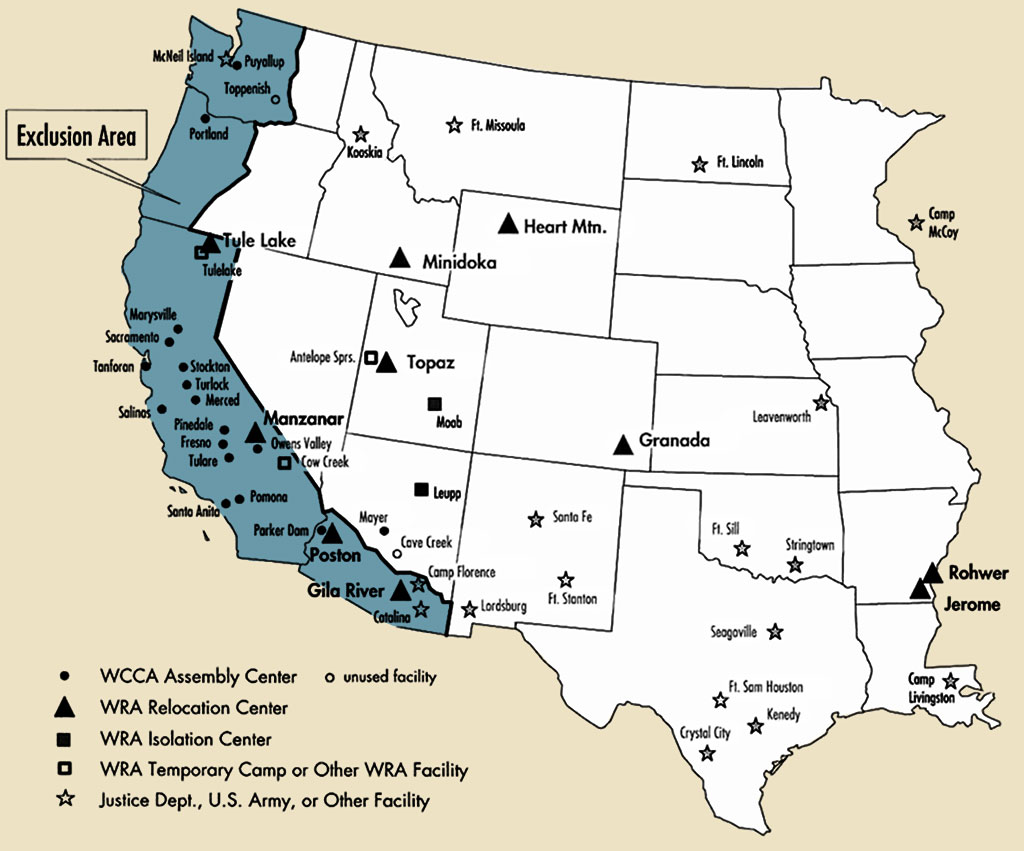
\includegraphics[width=1.0\textwidth]{../figures/PioCrtInternmentMap.jpg}
  \label{fig:internmentmap}
  \caption*{Source: \href{https://pioneercourthouse.org/gallery-Japanese-American-Internment.html}{Pioneer Courthouse Galleries}}
\end{figure}

\begin{figure}
  \centering
  \caption{Map of 1940 Japanese Population Distribution}
  \includegraphics[width=1.0\textwidth]{../figures/1940_map.pdf}
  \label{fig:1940JAmap}
\end{figure}

\begin{figure}
  \caption{Counts of interned persons by age and WRA camp}
  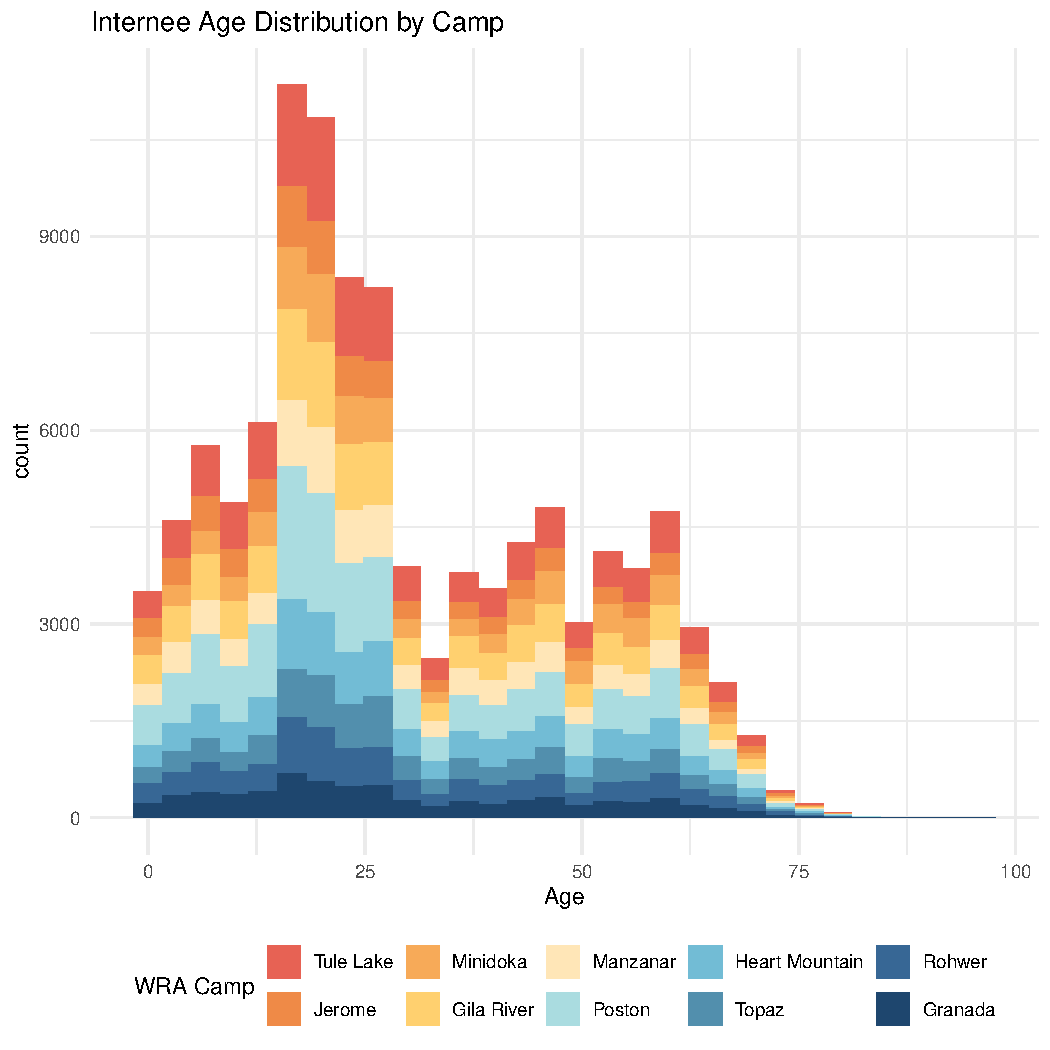
\includegraphics[width=0.6\textwidth]{../figures/internee-age_plot.pdf}
  \footnotesize \\
  Data from the WRA internment camp records on the ages of interned Japanese people in 1942
  infered from their reported birth year. 
  The counts of people in each of the ten internment camps created by the WRA are based on the initial camp they were placed in 
  after being moved from the temporary assembly centers.
  \label{fig:internee-ages}
\end{figure}

\begin{figure}
  \label{fig:intern_map}
  \centering
  \caption{Proportion of 1940 Japanese population interned vs. `Evacuation areas' in 1942}
  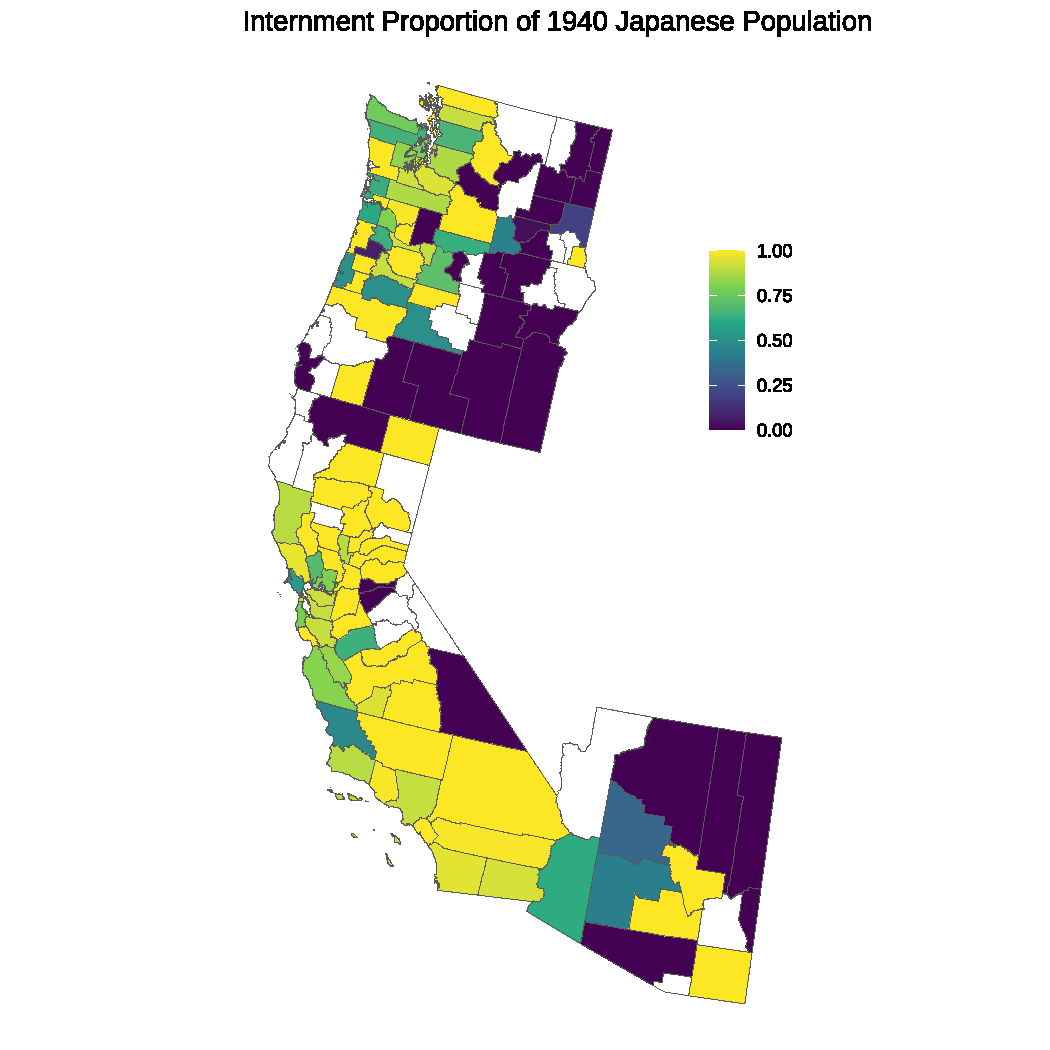
\includegraphics[width=\textwidth]{../figures/pr_interned_map.pdf} \\
  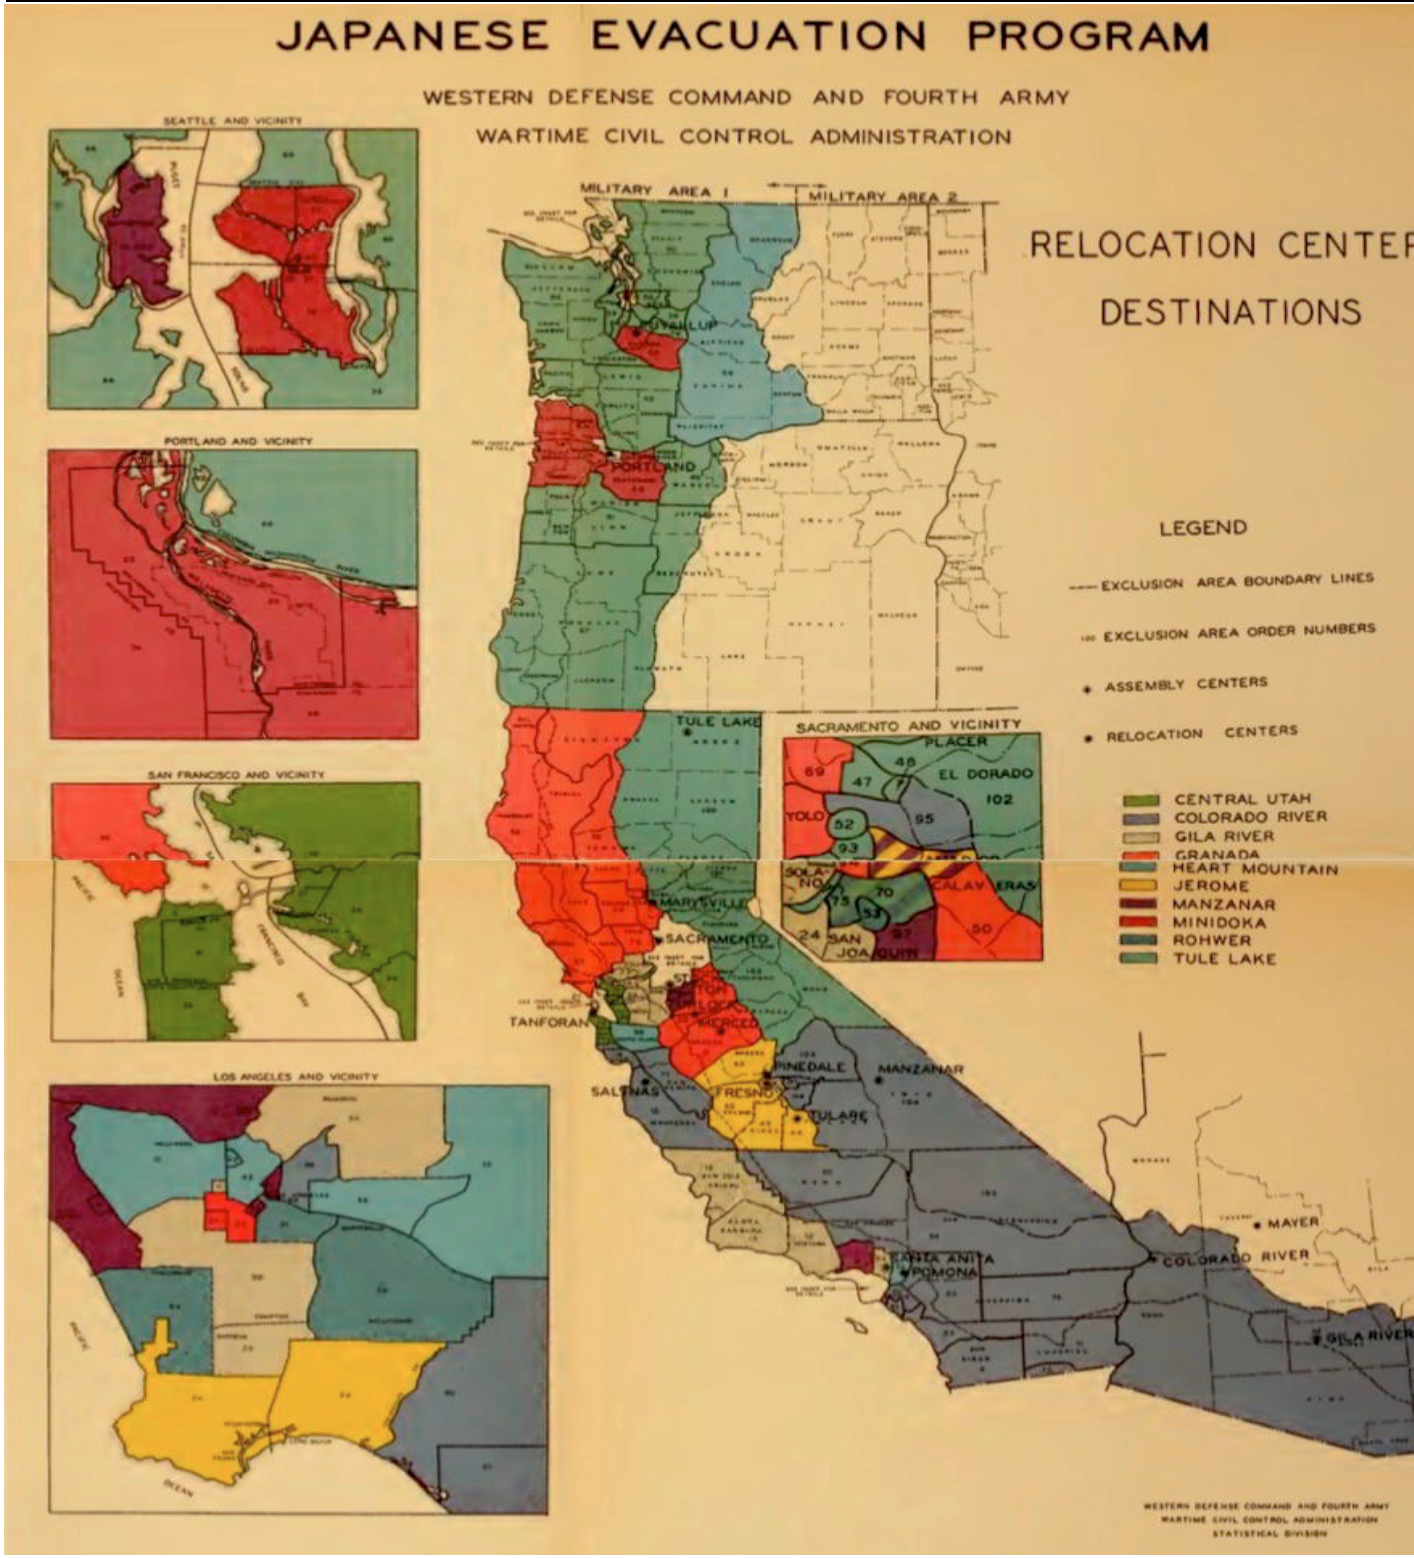
\includegraphics[height=5cm]{../figures/WRAzonesmap.png} \\
  \footnotesize
  Interned proportions are calculated as the number of internees from the county divided by the county's Japanese population in the 1940 full-count census.
  Counties in white had zero Japanese respondents in the 1940 census.
  The map on the below comes from the 1942 Western Defense Command's Final Report \citep{dewittjohnl.FinalReportJapanese1943}
  and shows in color the evacuation areas along the West Coast.
\end{figure}

\begin{figure}
  \label{fig:pr_intern}
  \caption{Counts of linked individuals by their estimated internment `probability'}
  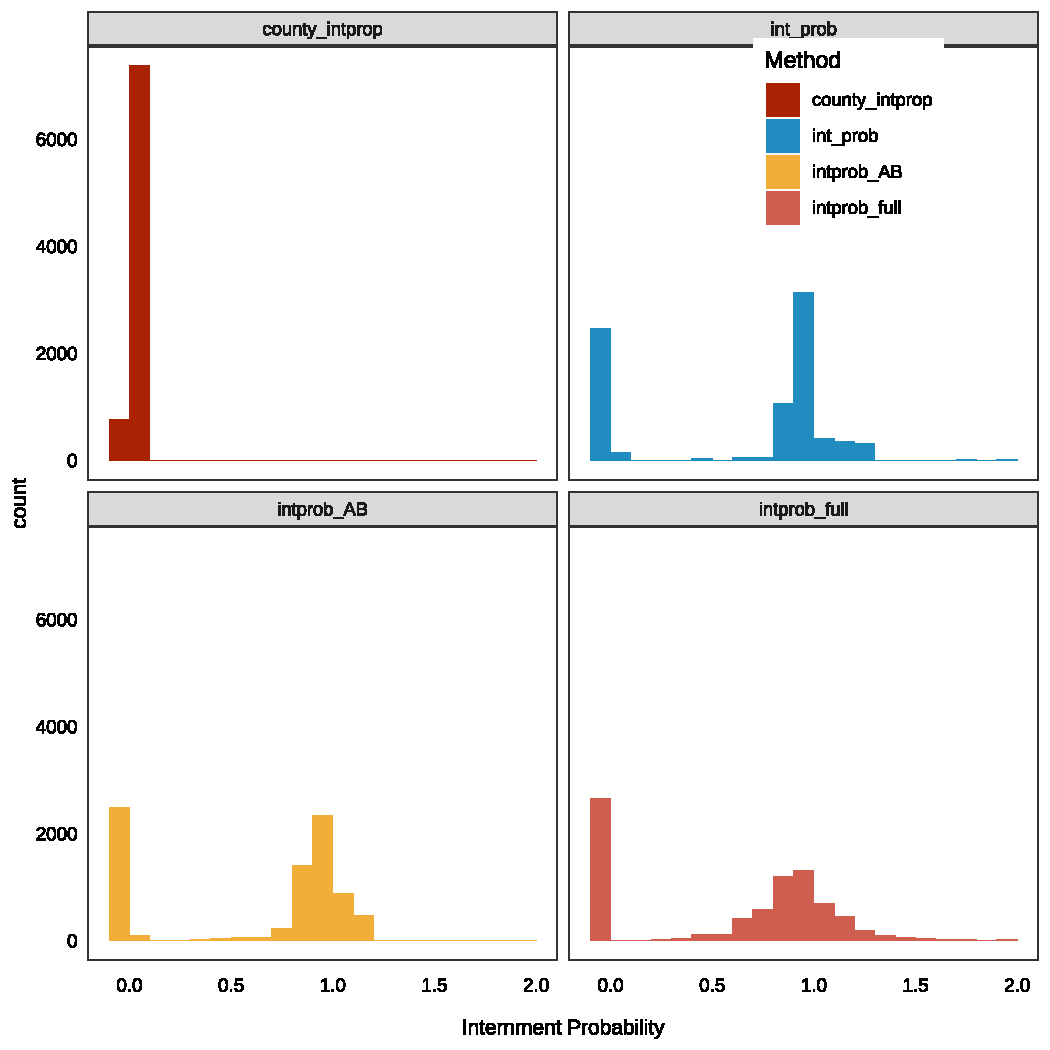
\includegraphics[width=.8\textwidth]{../figures/pr_intern_plot.pdf} \\
  \footnotesize
  This figure includes all Japanese and Chinese individuals who are linked across the 1940 and 1950 censuses
  in version 1.2 of the IPUMS MLP project.
  An individual's probability of being an internee is estimated as the ratio of interned people to the 
  number of people in the 1940 full-count census who have the same county and demographics.
  My cutoff for categorizing a person in the linked records as a likely internee is shown by the vertical line at 0.5.
\end{figure}


\begin{figure}
  \label{fig:wageeffect}
  \caption{Interned Japanese men experienced higher earnings growth than non-interned men.}
  \centering
  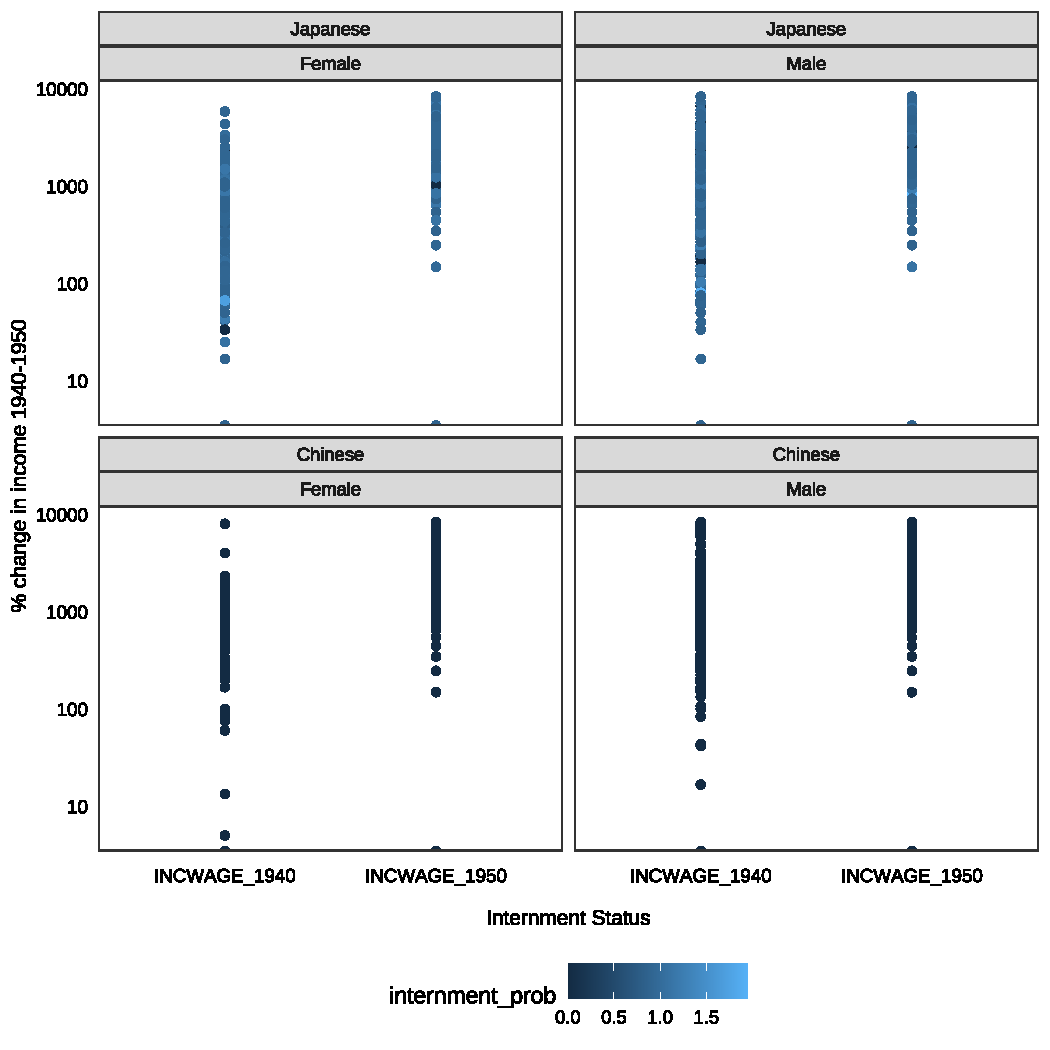
\includegraphics[width=\textwidth]{../figures/INCWAGE_plot.pdf} \\
  \footnotesize
  Interned proportions are calculated as the number of internees from the county divided by the county's Japanese population in the 1940 full-count census.
  Counties in white had zero Japanese respondents in the 1940 census.
  The map on the below comes from the 1942 Western Defense Command's Final Report \citep{dewittjohnl.FinalReportJapanese1943}
  and shows in color the evacuation areas along the West Coast.
\end{figure}

\section*{Tables}

\input{../tables/balance_stats.tex}\label{tbl:bal-stat}

\begin{table}[ht]
  \caption{Top 20 county origins of internees}
  \setlength{\tabcolsep}{4pt}
  \begin{tabular}{|ll|r|r|r|r|r|r|r|r|r|r|r|}
    \hline
    state & county & Jer & Manz & Post & Gila & Tule & Mind & Topz & HrtM & Grnd & Rhwr & Total \\ 
    \hline
    CA & LA & 3049 & 8879 & 2780 & 4851 & 360 &  28 &  62 & 6342 & 2837 & 4331 & 33520 \\ 
    WA & King &  &   1 &   8 &  20 & 2679 & 5852 &   8 &  18 &   6 &   6 & 8598 \\ 
    CA & Sac. & 965 & 376 & 664 & 401 & 4841 &  10 &  19 &   6 & 487 &  58 & 7827 \\ 
    CA & Fresno & 1942 &  25 & 1591 & 1936 &  37 &   8 &  20 &   1 &  23 &  37 & 5620 \\ 
    CA & S. Joaquin &   4 & 160 &  18 & 779 & 356 &  31 &  22 &   3 &  27 & 3511 & 4912 \\ 
    CA & S. Francisco &  59 &  81 &  63 & 174 & 225 &   6 & 3359 & 671 &  74 &  80 & 4792 \\ 
    CA & Alameda &  60 &  20 &  95 & 328 & 300 &  16 & 3635 & 111 &  77 &  51 & 4694 \\ 
    CA & S. Clara &  57 &  16 & 467 & 207 & 219 &  & 134 & 2502 &  50 &  16 & 3669 \\ 
    OR & Multnomah &  &   1 &   1 &  & 308 & 1864 &   1 &  66 &   1 &  & 2242 \\ 
    CA & Tulare & 199 &   4 & 1947 &  25 &   5 &   6 &   9 &   1 &   2 &   4 & 2202 \\ 
    CA & S. Diego &  25 &  38 & 1877 &  17 &   2 &   4 &   1 &  19 &  11 &   3 & 1997 \\ 
    WA & Pierce &  &   3 &  &  & 938 & 999 &  &   4 &  &   2 & 1946 \\ 
    CA & S. Barbara &  38 &  16 &  44 & 1767 &  16 &   1 &   7 &  23 &   6 &  20 & 1938 \\ 
    CA & Orange &  28 &  78 & 1611 &  57 &  10 &  &   3 &  17 &  10 &  41 & 1855 \\ 
    CA & Monterey &  44 &   8 & 1490 &  73 & 125 &   3 &  25 &   7 &  37 &  10 & 1822 \\ 
    CA & Placer &   3 &  &  10 &  & 1746 &   3 &   1 &   1 &   2 &   1 & 1767 \\ 
    CA & Imperial &  &   7 & 1486 &  16 &   2 &  &   2 &  11 &  &   6 & 1530 \\ 
    CA & S. Cruz &  23 &  & 1203 &  46 &  88 &   1 &   1 &  16 &  13 &   7 & 1398 \\ 
    CA & Kern & 332 &  13 & 821 &  16 &   9 &  10 &  10 &   2 &  13 &  15 & 1241 \\ 
    CA & Yolo &   1 &   1 &  10 & 120 & 348 &  &  &  & 626 &  & 1106 \\ 
     \hline
  \end{tabular}
  \footnotesize
  Numbers represent of count of internees who came from each county who were initially placed in one of the ten WRA camps.
  The camp name abbreviations in the table correspond to Jerome, Manzanar, Poston, Tule Lake, Minidoka, Topaz, Heart Mountain, Granada, and Rohwer.
  The Total column is the sum of all internees from the county across all camps.
\end{table}
    \label{tbl:cmp-cty}

\begin{table}[htbp]
   \caption{\label{tbl:reg1} Earning effects of internment}
   \bigskip
   \centering
   \begin{tabular}{lcccc}
      \toprule
       & \multicolumn{4}{c}{Income in 1950}\\
                                   & (1)     & (2)             & (3)             & (4)\\  
      \midrule 
      Internment Status            & -42.07  & 232.4$^{***}$   & 250.7$^{***}$   & 80.90\\   
                                   & (36.02) & (60.49)         & (59.86)         & (91.11)\\   
      Age                          &         & 33.30$^{***}$   & 12.45           & 11.22$^{**}$\\   
                                   &         & (7.837)         & (8.210)         & (4.786)\\   
      Age square                   &         & -0.5353$^{***}$ & -0.3143$^{***}$ & -0.3024$^{***}$\\   
                                   &         & (0.0808)        & (0.0835)        & (0.0461)\\   
      Male                         &         & 645.4$^{***}$   & 487.5$^{***}$   & 488.3$^{***}$\\   
                                   &         & (33.47)         & (35.14)         & (17.22)\\   
      Japanese                     &         & -210.0$^{***}$  & -246.2$^{***}$  & -98.45\\   
                                   &         & (63.93)         & (64.55)         & (88.69)\\   
      Income in 1940               &         &                 & 0.2409$^{***}$  & 0.2334$^{***}$\\   
                                   &         &                 & (0.0189)        & (0.0218)\\   
       \\
      Standard-Errors & \multicolumn{3}{c}{IID} & State$_{1940}$ \\ 
      Observations                 & 8,136   & 8,136           & 8,136           & 8,136\\  
      R$^2$                        & 0.00017 & 0.07616         & 0.10227         & 0.10882\\  
      Within R$^2$                 &         &                 & 0.08326         & 0.07855\\  
       \\
      Education fixed effects      &         &                 & $\checkmark$    & $\checkmark$\\   
      State$_{1940}$ fixed effects &         &                 &                 & $\checkmark$\\   
      \bottomrule
   \end{tabular}
\end{table}\label{tbl:reg1}

\begin{table}[htbp]
   \caption{\label{tbl:reg2} Employment and occupation effects}
   \begin{adjustbox}{width = \textwidth, center}
      \begin{tabular}{lccccc}
         \toprule
                               & Employed        & Hours worked    & Weeks worked    & Occ. score      & Occ. change\\  
                               & (1)             & (2)             & (3)             & (4)             & (5)\\  
                               &  Logit          & OLS             & OLS             & OLS             & Logit\\  
         \midrule 
         % (Intercept)           & -3.402$^{***}$  & -4.282          & 6.322$^{***}$   & 13.05$^{***}$   & -1.898$^{***}$\\   
         %                       & (0.2640)        & (3.084)         & (1.029)         & (2.171)         & (0.2156)\\   
         Internment Status     & -0.0138         & -1.504          & -0.9339         & 0.0739          & -0.5367$^{***}$\\   
                               & (0.1282)        & (1.040)         & (1.150)         & (0.9624)        & (0.2025)\\   
         Age                   & 0.1633$^{***}$  & 1.156$^{***}$   & 0.8436$^{***}$  & 0.0804          & 0.0576$^{***}$\\   
                               & (0.0125)        & (0.1481)        & (0.0421)        & (0.0914)        & (0.0089)\\   
         Age square            & -0.0022$^{***}$ & -0.0167$^{***}$ & -0.0135$^{***}$ & -0.0037$^{***}$ & -0.0004$^{***}$\\   
                               & (0.0001)        & (0.0014)        & (0.0004)        & (0.0009)        & ($9.26\times 10^{-5}$)\\    
         Male                  & 2.245$^{***}$   & 20.79$^{***}$   & 16.78$^{***}$   & 6.941$^{***}$   & -0.9214$^{***}$\\   
                               & (0.0267)        & (0.5576)        & (0.3428)        & (0.3454)        & (0.0542)\\   
         Japanese              & 0.5674$^{***}$  & 4.858$^{***}$   & 4.574$^{***}$   & -2.481$^{**}$   & 0.1879\\   
                               & (0.1319)        & (1.198)         & (1.407)         & (1.070)         & (0.1769)\\   
         Hours worked$_{1940}$ &                 & 0.1089$^{***}$  &                 &                 &   \\   
                               &                 & (0.0102)        &                 &                 &   \\   
         Weeks worked$_{1940}$ &                 &                 & 0.1355$^{***}$  &                 &   \\   
                               &                 &                 & (0.0089)        &                 &   \\   
         Occ. score$_{1940}$        &                 &                 &                 & 0.2649$^{***}$  &   \\   
                               &                 &                 &                 & (0.0075)        &   \\   
          \\
         Observations          & 8,136           & 8,136           & 8,136           & 8,136           & 8,136\\  
         Squared Correlation   & 0.25011         & 0.25589         & 0.25521         & 0.23167         & 0.06235\\  
         Pseudo R$^2$          & 0.20794         & 0.03173         & 0.03247         & 0.03232         & 0.05077\\  
         BIC                   & 8,420.4         & 73,447.2        & 71,494.9        & 64,251.3        & 9,449.2\\  
         \bottomrule
      \end{tabular}
   \end{adjustbox}
   {\footnotesize
   \emph{Note:}
   * = significant at the 10\% level,
   ** = 5\%, and
   *** = 1\%. \\
   Estimates of predicted internment status on 
   five different labor market outcome dependent variables,
   all measured in 1950 census.
   Column (1) reports results from a logit model on indicator for whether individual is employed in 1950.
   Columns (2) through (4) report OLS regression results 
   for number of hours worked in the previous week,
   weeks worked in the previous year,
   and a ranking of occupations based on median earnings of all 1950 census respondents in the same occupation.
   These three columns also control for the equivalent version of each dependent variable,
   but reported in the previous 1940 census for that same linked individual.
   Column (4) reports logit regression results on an indicator for whether
   the linked individual's reported occupation in 1950 was different from their 1940 one. \\
   \emph{Sources:} 1940-1950 Census, IPUMS Multigenerational Longitudinal Panel,
   and WRA records.
   }
\end{table}\label{tbl:reg2}

\end{document}